\documentclass[border=5pt]{standalone}
\usepackage{pgfplots}
\pgfplotsset{compat=1.18}

\begin{document}
	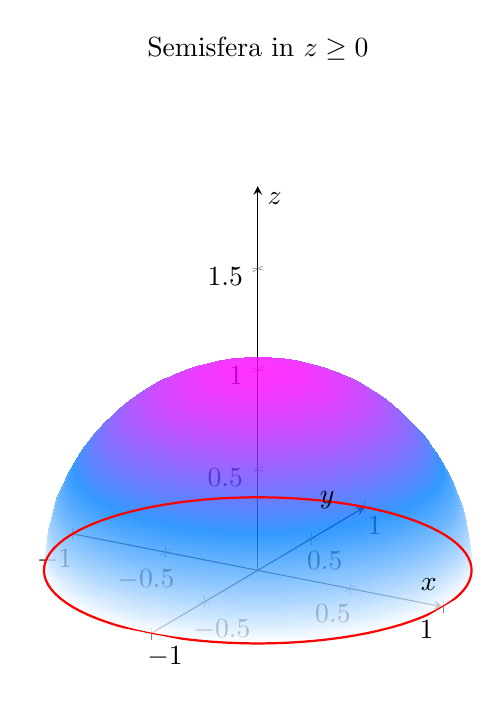
\begin{tikzpicture}
		\begin{axis}[
			width=9cm, height=9cm,
			view={30}{20},
			axis lines=center,
			axis equal,
			xlabel={$x$}, ylabel={$y$}, zlabel={$z$},
			zmin=0,
			title={Semisfera in $z \ge 0$},
			]
			
			% Superficie della semisfera
			% Coordinate sferiche: phi in [0,pi/2] (solo z>=0), theta in [0, 2*pi]
			% x = sin(phi)*cos(theta)
			% y = sin(phi)*sin(theta)
			% z = cos(phi)
			\addplot3[
			surf,
			shader=interp,
			colormap/cool,
			opacity=0.8,
			samples=40,
			domain=0:90,        % phi in gradi [0°, 90°]
			y domain=0:360,     % theta in gradi [0°, 360°]
			z buffer=sort,
			]
			(
			{sin(x)*cos(y)},    % x
			{sin(x)*sin(y)},    % y
			{cos(x)}            % z
			);
			
			% Bordo (cerchio z=0, raggio=1)
			\addplot3[
			thick,
			red,
			domain=0:360,
			samples=100,
			]
			(
			{cos(x)},   % x
			{sin(x)},   % y
			{0}         % z = 0
			);
			
		\end{axis}
	\end{tikzpicture}
\end{document}
